% Figure 2: Stability profile across five comparison levels and panel scoring.
% Horizontal bar chart; one \addplot per bar to allow per-bar fill color.
% Compile with: pdflatex (pgfplots >= 1.16, xcolor loaded by acmart)

\begin{figure}[t]
  \centering
  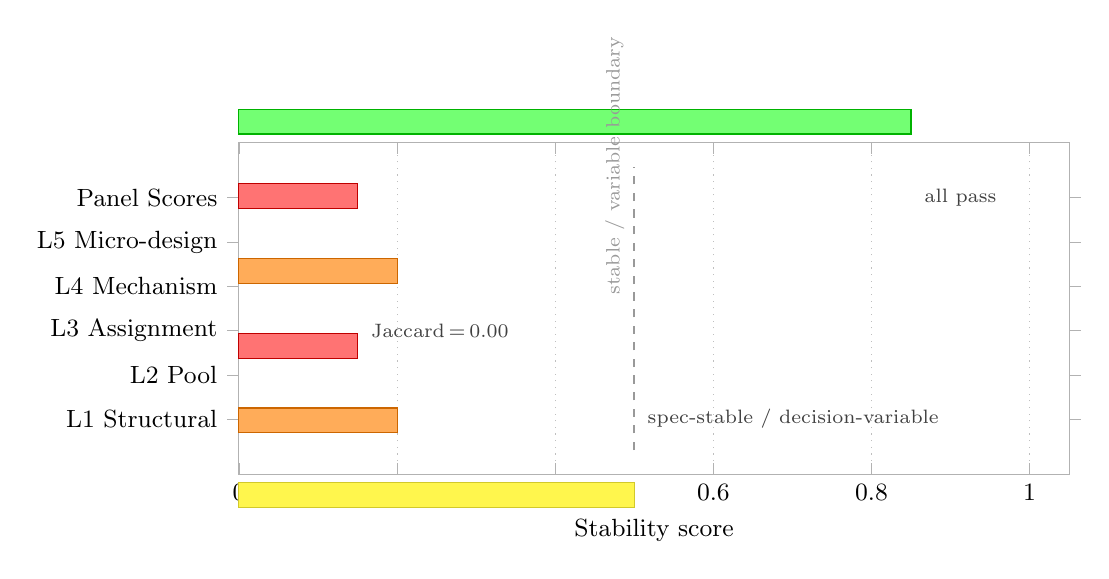
\begin{tikzpicture}
    \begin{axis}[
      % --- layout ---
      xbar,                          % horizontal bars
      width  = \columnwidth,
      height = 5.8cm,
      bar width = 9pt,
      % --- axes ---
      xmin = 0, xmax = 1.05,
      xtick = {0, 0.2, 0.4, 0.6, 0.8, 1.0},
      xticklabel style = {font=\small},
      xlabel = {Stability score},
      xlabel style = {font=\small},
      % y-axis: six named categories, bottom-to-top order matches data order
      ytick = {1,2,3,4,5,6},
      yticklabels = {
        {L1 Structural},
        {L2 Pool},
        {L3 Assignment},
        {L4 Mechanism},
        {L5 Micro-design},
        {Panel Scores}
      },
      yticklabel style = {font=\small, align=right},
      ymin = 0.3, ymax = 6.7,
      % --- grid ---
      xmajorgrids = true,
      grid style  = {dotted, gray!50},
      % --- general style ---
      enlarge y limits = {abs=0.55},
      axis line style  = {gray!60},
      tick style       = {gray!60},
      clip = false,       % allow annotations outside the plot area
    ]

    % ------------------------------------------------------------------
    % One \addplot per bar so each can carry its own fill color.
    % Coordinates: (score, y-index)
    % ------------------------------------------------------------------

    % L1 Structural — 0.50 — yellow (partial stability)
    \addplot[xbar, fill=yellow!70, draw=yellow!80!black, bar width=9pt]
      coordinates {(0.50, 1)};

    % L2 Pool — 0.20 — orange (low stability)
    \addplot[xbar, fill=orange!65, draw=orange!80!black, bar width=9pt]
      coordinates {(0.20, 2)};

    % L3 Assignment — 0.15 — red (very low stability)
    \addplot[xbar, fill=red!55, draw=red!75!black, bar width=9pt]
      coordinates {(0.15, 3)};

    % L4 Mechanism — 0.20 — orange (low stability)
    \addplot[xbar, fill=orange!65, draw=orange!80!black, bar width=9pt]
      coordinates {(0.20, 4)};

    % L5 Micro-design — 0.15 — red (very low stability)
    \addplot[xbar, fill=red!55, draw=red!75!black, bar width=9pt]
      coordinates {(0.15, 5)};

    % Panel Scores — 0.85 — green (high stability)
    \addplot[xbar, fill=green!55, draw=green!70!black, bar width=9pt]
      coordinates {(0.85, 6)};

    % ------------------------------------------------------------------
    % Reference line: stable/variable boundary at x = 0.5
    % ------------------------------------------------------------------
    \draw[dashed, gray!80, thick]
      (axis cs:0.5, 0.3) -- (axis cs:0.5, 6.7);
    \node[above, font=\scriptsize, gray!80, rotate=90, anchor=south]
      at (axis cs:0.50, 6.72) {stable / variable boundary};

    % ------------------------------------------------------------------
    % Bar annotations (placed to the right of each bar)
    % ------------------------------------------------------------------

    % L1: spec-stable / decision-variable
    \node[right, font=\scriptsize, text=black!75]
      at (axis cs:0.50, 1) {\,spec-stable / decision-variable};

    % L3: Jaccard = 0.00
    \node[right, font=\scriptsize, text=black!75]
      at (axis cs:0.15, 3) {\,Jaccard\,=\,0.00};

    % Panel Scores: all pass checkmark
    \node[right, font=\scriptsize, text=black!75]
      at (axis cs:0.85, 6) {\,all pass \checkmark};

    \end{axis}
  \end{tikzpicture}

  \caption{Stability scores across the five comparison levels and panel
  scoring, where 1.0 indicates full stability and 0.0 indicates full
  variability. Levels~1--5 all fall below the stable/variable boundary
  (dashed), while panel score stability (0.85) is well above it.
  Level~1 is partially stable because the specification constrains the
  decision space but does not fully determine the output.}
  \label{fig:stability}
\end{figure}
